\section{Results}

\subsection{Overall research output}
Since the release of the "Nudge" by Thaler and Sunstein in 2009, the concept of nudges gained more and more interest in several research streams and domains...

For reasons of overview, the domain names are coded. The complete coding of the domain names is available in the appendix on table \ref{table:domain-coding} as well as in the abbreviation section.

\begin{table}[htbp]
\centering
\small
\begin{tabular}{l|cccccccccc}
\textbf{Publishing year} & \textbf{CCH} & \textbf{EDU} & \textbf{FIN} & \textbf{HEA} & \textbf{PSB} & \textbf{SUS} & \textbf{TRA} & \textbf{SCP} & \textbf{GOV} & \textbf{MISC} \\ \hline
2011 (1) & 1 & 0 & 0 & 0 & 0 & 0 & 0 & 0 & 0 &  0 \\
2012 (1) & 0 & 0 & 0 & 0 & 0 & 0 & 0 & 0 & 0 & 1 \\
2013 (0) & 0 & 0 & 0 & 0 & 0 & 0 & 0 & 0 & 0 & 0 \\
2014 (5) & 4 & 0 & 0 & 0 & 0 & 0 & 1 & 0 & 0 & 0 \\
2015 (3) & 0 & 0 & 1 & 2 & 0 & 0 & 0 & 0 & 0 & 0 \\
2016 (7) & 3 & 0 & 0 & 1 & 1 & 1 & 0 & 1 & 0 & 0 \\
2017 (10) & 6 & 0 & 0 & 0 & 2 & 1 & 0 & 1 & 0 & 0 \\
2018 (9) & 5 & 0 & 0 & 1 & 0 & 1 & 0 & 1 & 0 & 1 \\
2019 (1) & 1 & 0 & 0 & 0 & 0 & 0 & 0 & 0 & 0 & 0 \\ \hline
\textbf{Total (37)} & 20 & 0 & 1 & 4 & 3 & 3 & 1 & 3 & 0 & 2
\end{tabular}
\caption{Overall research output across domains}
\label{table:research-output}
\end{table}

%%%%%%%%%%%%%%%%%%%%%%%

\subsection{Research type and methods}
Identified articles categorized based on the Alavi and Carlson's research classification scheme (\cite{alavi_review_1992}).

\begin{figure}[h!]
    \centering
    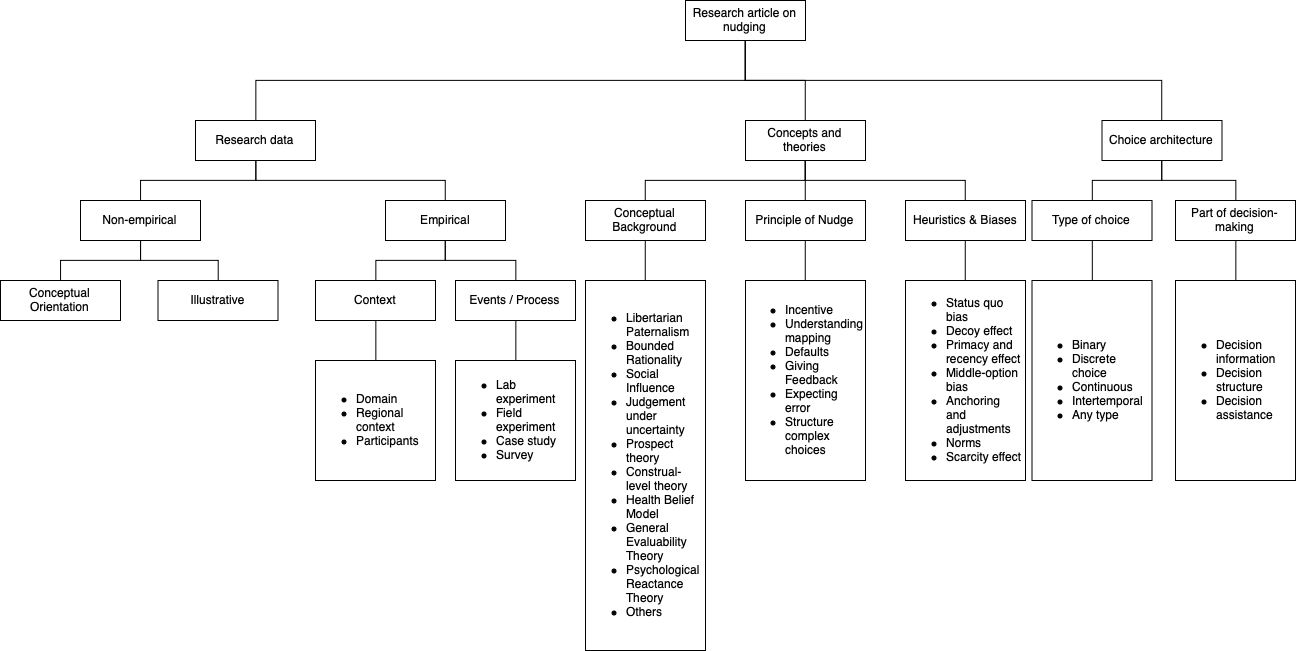
\includegraphics[width=1.0\textwidth]{analysis.png}
    \caption{Classification of findings}
    \label{fig:analysis}
\end{figure}


\subsubsection{Non-empirical}
\begin{table}[htbp]
\centering
\begin{tabular}{l|ccc}
\textbf{Non-empirical research} & \textbf{CCH} & \textbf{SCP} & \textbf{MISC} \\ \hline
Literature review (1) & 1 & 0 & 0 \\
Conceptual (2) & 1 & 1 & 0 \\
Literature review and conceptual (4) & 3 & 0 & 1 \\ \hline
\textbf{Total (7)} & 5 & 1 & 1
\end{tabular}
\caption{Non-empirical research across domains}
\label{table:non-empirical}
\end{table}

Sources:
\cite{cao_economic_2018} \\
\cite{yoo_consumer_2018} \\
\cite{gamliel_average_2017} \\
\cite{munscher_review_2016} \\
\cite{broniarczyk_decision_2014} \\
\cite{lades_impulsive_2014} \\
\cite{dolan_influencing_2012} \\
\paragraph{Literature review}
\paragraph{Conceptual}

\subsubsection{Empirical}
\begin{table}[htbp]
\small
\centering
\begin{tabular}{p{3.6cm}|cccccccccc}
\textbf{Empirical research} & \textbf{CCH} & \textbf{EDU} & \textbf{FIN} & \textbf{HEA} & \textbf{PSB} & \textbf{SUS} & \textbf{TRA} & \textbf{SCP} & \textbf{GOV} & \textbf{MISC} \\ \hline
Lab experiment (15) & 10 & 0 & 0 & 2 & 1 & 1 & 0 & 0 & 0 & 1 \\
Field experiment (5) & 2 & 0 & 0 & 1 & 1 & 1 & 0 & 0 & 0 & 0 \\
Lab experiment and field experiment (1) & 0 & 0 & 0 & 0 & 1 & 0 & 0 & 0 & 0 & 0 \\
Lab experiment and survey (3) & 2 & 0 & 0 & 0 & 0 & 0 & 0 & 1 & 0 & 0 \\
Survey (5) & 2 & 0 & 1 & 0 & 0 & 0 & 1 & 1 & 0 & 0 \\
Case Study (1) & 0 & 0 & 0 & 1 & 0 & 0 & 0 & 0 & 0 & 0 \\
Case Study, survey and lab experiment (1) & 0 & 0 & 0 & 0 & 1 & 0 & 0 & 0 & 0 & 0 \\ \hline
\textbf{Total (31)} & 16 & 0 & 1 & 4 & 4 & 2 & 1 & 2 & 0 & 1
\end{tabular}
\caption{Empirical research across domains}
\label{table:empirical}
\end{table}

\begin{table}[htbp]
\centering
\small
\begin{tabular}{p{3.6cm}|cccc}
\textbf{Empirical research} & \multicolumn{1}{l}{\textbf{\begin{tabular}[c]{@{}l@{}}Decision \\ Information\end{tabular}}} & \multicolumn{1}{l}{\textbf{\begin{tabular}[c]{@{}l@{}}Decision \\ structure\end{tabular}}} & \multicolumn{1}{l}{\textbf{\begin{tabular}[c]{@{}l@{}}Decision \\ assistance\end{tabular}}} & \multicolumn{1}{l}{\textbf{Combination}} \\ \hline
Lab experiment (15) & 9 & 5 & 1 & 0 \\
Field experiment (5) & 0 & 1 & 1 & 3 \\
Lab experiment and field experiment (1) & 0 & 1 & 0 & 0 \\
Lab experiment and survey (3) & 1 & 2 & 0 & 0 \\
Survey (5) & 2 & 0 & 0 & 3 \\
Case Study (1) & 1 & 0 & 0 & 0 \\
Case Study, survey and lab experiment (1) & 1 & 0 & 0 & 0 \\ \hline
\textbf{Total (31)} & 12 & 9 & 2 & 6
\end{tabular}
\caption{Empirical research across parts of the choice architecture}
\label{tabel:empirical-choice-arch}
\end{table}

\paragraph{Case Study}
\paragraph{Survey}
\paragraph{Lab Experiment}
\paragraph{Field Experiment}

\subsubsection{Context of Use}
\paragraph{Participants}
\paragraph{Location}
\paragraph{Domain}

%%%%%%%%%%%%%%%%%%%%%%%

\subsection{Theories and concepts used to study nudges}

\subsubsection{Principle of Nudge}
\paragraph{Incentive}
\paragraph{Understanding mapping}
\paragraph{Defaults}
\paragraph{Giving Feedback}
\paragraph{Expecting Error}
\paragraph{Structure complex choices}

\subsubsection{Conceptual Background}
\paragraph{Libertarian Paternalism}
\paragraph{Bounded Rationality}
\paragraph{Social Influence}
\paragraph{Judgment under uncertainty}
\paragraph{Prospect theory}
\paragraph{Construal-level theory}
\paragraph{Health Belief Model}
\paragraph{General Evaluability Theory}
\paragraph{Psychological Reactance Theory}
\paragraph{Others}

\subsubsection{Heuristics and biases}
\begin{table}[htbp]
\centering
\begin{tabular}{l|cccc}
\textbf{Heuristic / Bias} & \multicolumn{1}{l}{\textbf{\begin{tabular}[c]{@{}l@{}}Decision \\ information\end{tabular}}} & \multicolumn{1}{l}{\textbf{\begin{tabular}[c]{@{}l@{}}Decision \\ structure\end{tabular}}} & \multicolumn{1}{l}{\textbf{\begin{tabular}[c]{@{}l@{}}Decisions \\ assistance\end{tabular}}} & \multicolumn{1}{l}{\textbf{Combination}} \\ \hline
Status quo bias (5) & 0 & 5 & 0 & 0 \\
Decoy effect (1) & 0 & 1 & 0 & 0 \\
Primacy and recency effect (1) & 0 & 1 & 0 & 0 \\
Middle-option bias (0) & 0 & 0 & 0 & 0 \\
Anchoring and adjustments (1) & 1 & 0 & 0 & 0 \\
Norms (12) & 8 & 1 & 2 & 1 \\
Status quo bias and norms (1) & 0 & 1 & 0 & 0 \\
Scarcity effect (0) & 0 & 0 & 0 & 0 \\ \hline
\textbf{Total (21)} & 9 & 9 & 2 & 1
\end{tabular}
\caption{Heuristics used across parts of choice architectures}
\label{table:heuristics-choice}
\end{table}
\paragraph{Status Quo Bias}
\paragraph{Decoy Effect}
\paragraph{Primacy and Recency Effect}
\paragraph{Middle-option bias}
\paragraph{Anchoring and adjustments}
\paragraph{Norms}
\paragraph{Scarcity effect}

%%%%%%%%%%%%%%%%%%%%%%%

\subsection{Influence on the choice architecture and decision making}

\subsubsection{Type of choice}
\paragraph{Binary}
\paragraph{Discrete choice}
\paragraph{Continuous}
\paragraph{Any type of choice \& inter temporal}

\subsubsection{Choice architecture}
\begin{table}[htbp]
\centering
\small
\begin{tabular}{p{3.5cm}|cccccccccc}
\textbf{Choice Architecture} & \textbf{CCH} & \textbf{EDU} & \textbf{FIN} & \textbf{HEA} & \textbf{PSB} & \textbf{SUS} & \textbf{TRA} & \textbf{SCP} & \textbf{GOV} & \textbf{MISC} \\ \hline
Decision information (15) & 10 & 0 & 1 & 2 & 1 & 0 & 0 & 0 & 0 & 1 \\
Decision structure (10) & 4 & 0 & 0 & 0 & 2 & 2 & 0 & 2 & 0 & 0 \\
Decision assistance (3) & 2 & 0 & 0 & 1 & 0 & 0 & 0 & 0 & 0 & 0 \\
Combination (6) & 2 & 0 & 0 & 1 & 0 & 1 & 1 & 1 & 0 & 0 \\ \hline
\textbf{Total (34)} & 18 & 0 & 1 & 4 & 3 & 3 & 1 & 3 & 0 & 1
\end{tabular}
\caption{Choice architecture parts used across the domains}
\label{tabel:choice-arch-domains}
\end{table}
\paragraph{Decision information}
\subparagraph{Translate Information}
\subparagraph{Make information visible}
\subparagraph{Reference point}
\paragraph{Decision structure}
\subparagraph{Change defaults}
\subparagraph{Change effort}
\subparagraph{Change range or composition of options}
\subparagraph{Change consequences}
\paragraph{Decision assistance}
\subparagraph{Provide reminders}
\subparagraph{Facilitate commitment}






%General Content:
%The presentation of the literature review’s results is the main part of this seminar thesis. Identified concepts, research types, use cases and more will be presented and discussed step by step. The goal of this chapter is to provide a detailed explanation of the underlying concepts and insights of the examined literature. This could include sub chapters like:
%-	General information (number of articles, year of publishing, domain of journal)
%-	Research type (empirical, non-empirical, qualitative, quantitative)
%-	Field of use (IS Field, use case)
%-	Nudging principles and concepts (used biases, choices, design elements)
